\chapter{Introduction and Goals}

\section{Introduction}

This document intends to describe the low-level design of the SUM_DIAG module.  The scope of this document is to capture the implementation based on the requirements as defined in 
GB8002_AUTOSAR_Standard_Utility_Module_Specification.  For a better process and higher quality design, this can be seen as an extension to the before mentioned document. 

\subsection{System Purpose}

This document defines a set of standard software compositions which are referred to as GM Standardized Utility Modules (SUM). 
Use of the SUM modules allows for standardized specification of behavior requirements and expectations with respect to the interface to the software infrastructure (BSW Services). This allows functional software to be completely abstracted from 
the software infrastructure. SUM will be used to communicate a set of standardized implementations of the interactions between SW-C and BSW.
The Standard Utility Module, Diagnostic Application Service (SUM_DIAG), is a software composition located in the Application Layer of the standardized architecture of AUTOSAR.

Main Features:
\begin{itemize}
	\item Handling management of Manufacturer Enable Counter
	\item Verify preconditions to support Diagnostic Session Control service
	\item Verify preconditions to support Read Memory by Address service
	\item Verify preconditions to support Communication Control service
	\item Verify preconditions to support Dynamically Define Data Identifier service
	\item Multiple Tester Connectivity for verifying received diagnostic requests associated with individual diagnostic sessions
	\item Provide confirmation for Communication Control request
	\item Provide confirmation for Diagnostic Session Control request
	\item Provide confirmation for ControlDTCSetting 0x85 request
	\item Provide OTA_PSF status to SWC
	\item Provide status of MEC and Dcm Communication Mode Status to other SUMs, SW-Cs
\end{itemize}

\subsection{Document Purpose}

This document introduces the key ideas of the architecture of SUM_DIAG. Its intended audience comprises System Architects, Product Architects, Developers and Testers 
who need a rough understanding on the concepts of the product.

The document describes the product and its functionality on the component level, the interaction and communication between those components and the integration of ETAS 
wide shared components.

The document does not explain the components design in detail.

\section{Goals of the Architecture}

\subsection{Goals}

The main goals of the architecture are:

\begin{enumerate}
\item \textbf{Configurability}: The module has to be designed with the highest possible level of configurability, in order to be easy to adapt it in the future to changes on the standard or even in some project requirements.
\item \textbf{Maintainability}: The architecture of the component shall be clearly defined and easy to understand, in order to guarantee the maximum possible level of maintainability.
\item \textbf{Performance}: The component shall be designed in order to maximize run-time execution speed as well as minimize memory consumption.
\item \textbf{Correctness of Implementation}: The Detailed Design must to be aligned to the Architecture document.
\end{enumerate}

\section{Stakeholders}

\begin{figure}[h]
	\centering
		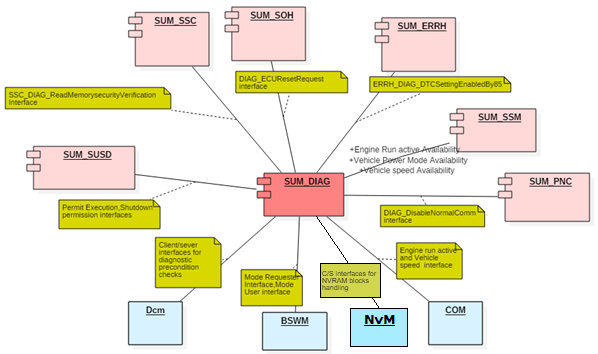
\includegraphics[width=15cm]{images/stakeholders}
	\caption{SUM_DIAG stakeholders}
\end{figure}

\section{Definitions, Acronyms and Abbreviations}

\input{generated/tables/definitions.tex}

\section{Referenced Documents}

\input{generated/tables/references.tex}